\begin{figure}
    \centering
    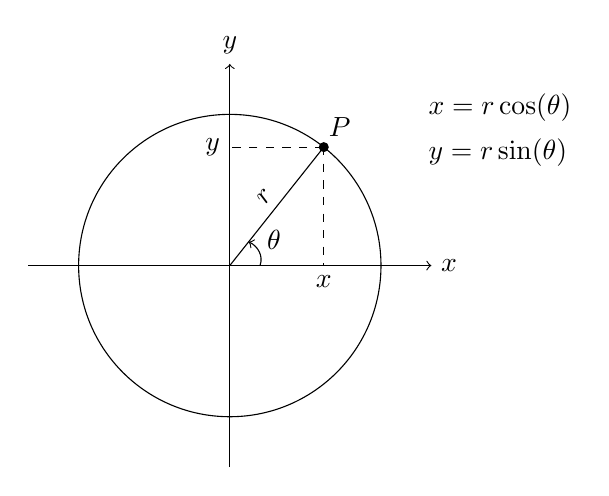
\begin{tikzpicture}[scale=.8]
	\draw [->] (-3.2,0) -- (3.2,0);
	\draw [->] (0,-3.2) -- (0,3.2);
	\draw (0,0) circle (2.4);
	\draw (0,0) -- (1.49186,1.87998);
	\draw [fill] (1.49186,1.87998) circle (.07);
	\draw [dashed] (1.49186,1.87998) -- (1.49186,0);
	\draw [dashed] (1.49186,1.87998) -- (0,1.87998);
	\node [right] at (3.2,0) {$x$};
	\node [above] at (0,3.2) {$y$};
	\node at (1.17*1.49186,1.17*1.87998) {$P$};
	\node [below] at (1.49186,0) {$x$};
	\node [left] at (0,1.87998) {$y$};
	\draw [->] (1.2*.4,0) to[out=70, in=-25] (1.2*.2486,1.2*.3133);
	\node at (.7,.4) {$\theta$};
	\node [above,rotate=51] at (.5*1.49186,.5*1.87998) {$r$};
	\node [right] at (3,2.5) {$x = r \cos(\theta)$};
	\node [right] at (3,1.8) {$y = r \sin(\theta)$};
	\end{tikzpicture}
    \caption{Kugle for enden af en snor, der roterer i en cirkelbevægelse.}
    \label{mat:fig:pol_koor}
\end{figure}

\section{Polære koordinater \& Trigonometri} \label{mat:sec:trig}
Forestil dig en kugle for enden af en snor, der roterer i
en cirkelbevægelse som i \cref{mat:fig:pol_koor}. Kuglen roterer i en to-dimensionalt plan. Til et bestemt tidspunkt befinder kulgen sig i punktet $P$. Når vi har lagt et koordinatsystem som på tegningen kan vi beskrive punket $P$ ved at angive dets $x$- og $y$-værdi. Disse koordinater ($x$ og $y$) kaldes \emph{kartesiske koordinater}. Det er muligt, at beskrive $P$ ved hjælp af andre koordinater. Man kunne også beskrive $P$ ved at angive afstanden $r$ fra centrum af koordinatsystemet, som kaldes \textit{origo}, og vinklen $\theta$ mellem $x$-aksen og linjen fra origo til $P$, se \cref{mat:fig:pol_koor}. Disse koordinater ($r$ og $\theta$) kaldes \emph{polære koordinater}.

\subsection{Frihedsgrader}
Fordelen ved polære koordinater kan ses, når vi tænker på at kuglen roterer. Til et senere tidspunkt har kuglen flyttet sig til et andet punkt på cirklen. I kartesiske koordinater vil det nye punkt have både en ny $x$- og $y$-værdi, men i polære koordinater vil vinklen, $\theta$, være ny, men radius, $r$, er uændret. I polære koordinater er det således kun ét koordinat, der ændres, når kuglen roterer rundt -- med andre ord skal vi bruge ét tal, til at fortælle os, hvor kuglen er til et bestemt tidspunkt. Et vigtigt begreb i fysik er antallet af \textit{frihedsgrader}, hvilket er det antal af informationer, der skal til for at beskrive noget bestemt. Systemet med kuglen i snoren har én frihedsgrad, da vinklen er den eneste nødvendige information. Antallet af frihedsgrader er det samme, uanset hvilket koordinatsystem man vælger, men hvis man arbejder med flere koordinater end frihedsgrader, så er koordinaterne også afhængige af hinanden, hvilket vi så med de kartesiske koordinater for kuglen.% I eksemplet med kuglen ses det at vi kan ændre $\theta$, uden at ændre $r$, men hvis vi ændrer $x$, så er vi også nød til at ændre $y$, for at blive på cirklen. De kartesiske koordinater er altså afhængige af hinanden.

\subsection{Trigonometri}
En ting er at kunne bruge polære koordinater, til at beskrive en bevægelse. For at det er brugbart, skal vi gerne kunne omregne dem til de kartesiske koordinater, hvor relationerne er:
%
\begin{equation} \label{mat:eq:kartesisk/polaer}
\begin{aligned}
    x &= r \cos(\theta), \\
    y &= r \sin(\theta), \\
    r &= \sqrt{x^2 + y^2}, \\
    \theta &= \tan^{-1}\left(\frac{y}{x}\right),
\end{aligned}
\end{equation}
%
hvor $\tan^{-1}(x)$ er den inverse funktion til tangens\footnote{Dvs. at $\tan^{-1} \left( \tan(x) \right) = \tan \left( \tan^{-1}(x) \right) = x$.}. I udtrykkene for $x$ og $y$ indgår henholdsvis funktionerne cosinus og sinus. De er defineret som på \cref{mat:fig:pol_koor}: $\theta$ angiver vinklen mellem $x$-aksen og et punkt, mens
%
\begin{align*}
    \cos(\theta) &= \text{$x$-koordinaten for punktet på cirklen med
	radius $r = 1$,}\\
    \sin(\theta) &= \text{$y$-koordinaten for punktet på cirklen med
	radius $r = 1$.}
\end{align*}
%
Disse funktioner er $2\pi$-periodiske, hvilket betyder at eksempelvis $\cos(\theta + 2\pi) = \cos(\theta)$, hvorfor det ikke ændrer noget at øge en vinkel med $2\pi$, som svarer til at gå en hel omgang rundt i cirklen\footnote{Dette er sandt, når man angiver vinkler i radianer, mens perioden for de trigonometriske funktioner er 360, hvis man arbejder i grader. På campen holder vi os til radianer, da det er hvad man ofte bruger.}. \\
Cosinus og sinus har også noget med trekanter at gøre. Hvis vi kigger på \cref{mat:fig:pol_koor} igen, ser vi, at den indeholder to retvinklede trekanter: $\bigtriangleup OxP$ og $\bigtriangleup OyP$, hvor $O$ betegner centrum. I retvinklede trekanter betegner man den længste side som hypotenusen og de to andre sider som kateter. Hypotenusen i de to trekanter i figuren er $r$, og de to kateter er $x = r \cos(\theta)$ og $y = r \cos(\theta)$. Vi kan altså lave en tegning, der illustrerer længderne i en retvinklet trekant, hvilket ses i \cref{mat:fig:trekant}.
%
\begin{figure}
    \centering
    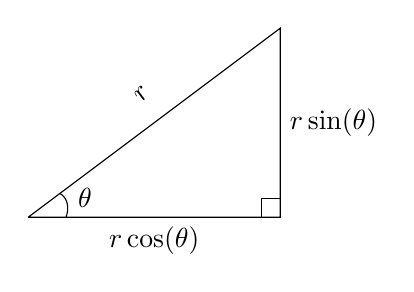
\begin{tikzpicture}[scale=.8]
	\draw [-] (0,0) -- (4,0) -- (4,3) -- (0,0);
	\draw [-] (.6,0) to[out=70, in=-30] (.5,.38);
	\node at (.9,.3) {$\theta$};
	\node [above,rotate=51] at (2,1.8) {$r$};
	\node [below] at (2,0) {$r \cos(\theta)$};
	\node [right] at (4,1.5) {$r \sin(\theta)$};
	\draw [-] (3.7,0) -- (3.7,.3) -- (4,.3);
	\end{tikzpicture}
    \caption{Retvinklet trekant, der viser sammenhængen mellem en vinkel og de tre sidelængder.}
    \label{mat:fig:trekant}
\end{figure}
%
Heraf følger, at cosinus og sinus er forholdet mellem to længder i den retvinklede trekant:
\begin{align} \label{mat:eq:trig}
    &\cos(\theta) = \frac{\text{hosliggende side}}{\text{hypotenusen}}\\
    &\sin(\theta) = \frac{\text{modstående side}}{\text{hypotenusen}}
\end{align}
Vi definerer også en funktion kaldet tangens:
\begin{align*}
    \tan(\theta) = \frac{\sin(\theta)}{\cos(\theta)} = \frac{\text{modstående side}}{\text{hosliggende side}}
\end{align*}
Hvis vi sætter $r=1$ får vi fra Pythagoras' sætning at
\begin{equation*}
    \cos^2 \theta + \sin^2 \theta = 1,
\end{equation*}
hvor vi har brugt notationen $\cos^2 \theta = (\cos(\theta))^2$ og
$\sin^2 \theta = (\sin(\theta))^2$.